% !TeX root = thesis.tex
%% evaluation.tex
%%

%% ==============
\chapter{Evaluation\label{ch:Evaluation}}
In this section, we evaluate the running time and behavior of our algorithms of Chapter~\ref{ch:Algorithm}. Our machine runs openSUSE Leap 15.3, has \SI{128}{\giga\byte} (8x\SI{16}{\giga\byte}) of \SI{2133}{\mega\hertz} DDR4 RAM, and a 4-core Intel Xeon E5-1630v3 CPU which runs at \SI{3.7}{\giga\hertz}. The code is written in Rust and compiled with cargo 1.64.0-nightly using the release profile with \texttt{lto~=~true} and \texttt{codegen-units~=~1}.

\subparagraph{Data.} Our data is a road network of Europe\footnote{\url{https://download.geofabrik.de/europe-latest.osm.pbf} of March 22, 2022} and of Germany\footnote{\url{https://download.geofabrik.de/europe/germany-latest.osm.pbf} of March 22, 2022} from Open Street Map (OSM). We extract the routing graph and parking nodes from the OSM data using a custom extension\footnote{\url{https://github.com/maxoe/RoutingKit}} of RoutingKit\footnote{\url{https://github.com/RoutingKit/RoutingKit}}. The obtained routing graph of Europe has $81.5$ million nodes and $190$ million edges. If not stated otherwise, our set $P$ of parking nodes in the European routing graph consists of \num{6796} nodes which were selected according to their OSM attributes. The routing graph of Germany has $12.5$ million nodes, $29.5$ million edges, and we selected \num{3222} nodes as parking nodes.

RoutingKit constructs the routing graph by filtering the OSM data using a rich set of attributes to determine which of the OSM objects can be used for driving with a car. The OSM objects types of importance are OSM nodes and OSM ways. An OSM node is a location with associated geographic coordinates and an OSM way is a polyline consisting of multiple OSM nodes. RoutingKit removes OSM nodes which are only used for modelling of the shape of roads to obtain the set of nodes for the routing graph. It then uses additional attributes to classify the OSM ways into categories with different assumed average speeds. The categorized OSM ways and their spatial length are used to determine driving times between the routing nodes which can then be used as the length function $\len$ of the routing graph. In our custom extension, we additionally extract parking nodes from the OSM data. The extraction again is based on attributes which indicate a designated parking location for heavy goods vehicles (HGV), i.e., if \texttt{hgv = "yes"} or \texttt{hgv = "designated"} or \texttt{access = "hgv"} is true. Figure~\ref{fig:parking_qgis} gives an overview over all extracted HGV parking locations. All following visualizations of spatial data in this chapter are obtained from the QGIS software\cite{qgisdevelopmentteam:2022}. It is apparent that in some areas in Europe there are a lot more parking areas marked as HGV parking than in others. In general, the location of designated HGV parking areas correlates with the location of highways. Figure \ref{fig:parking_central_europe__qgis} shows that especially in areas with many designated HGV parking locations, the structure of the highway network becomes visible.

\begin{figure}[hbtp]
	\centering
	\subfigure[Full HGV Parking Set]{
		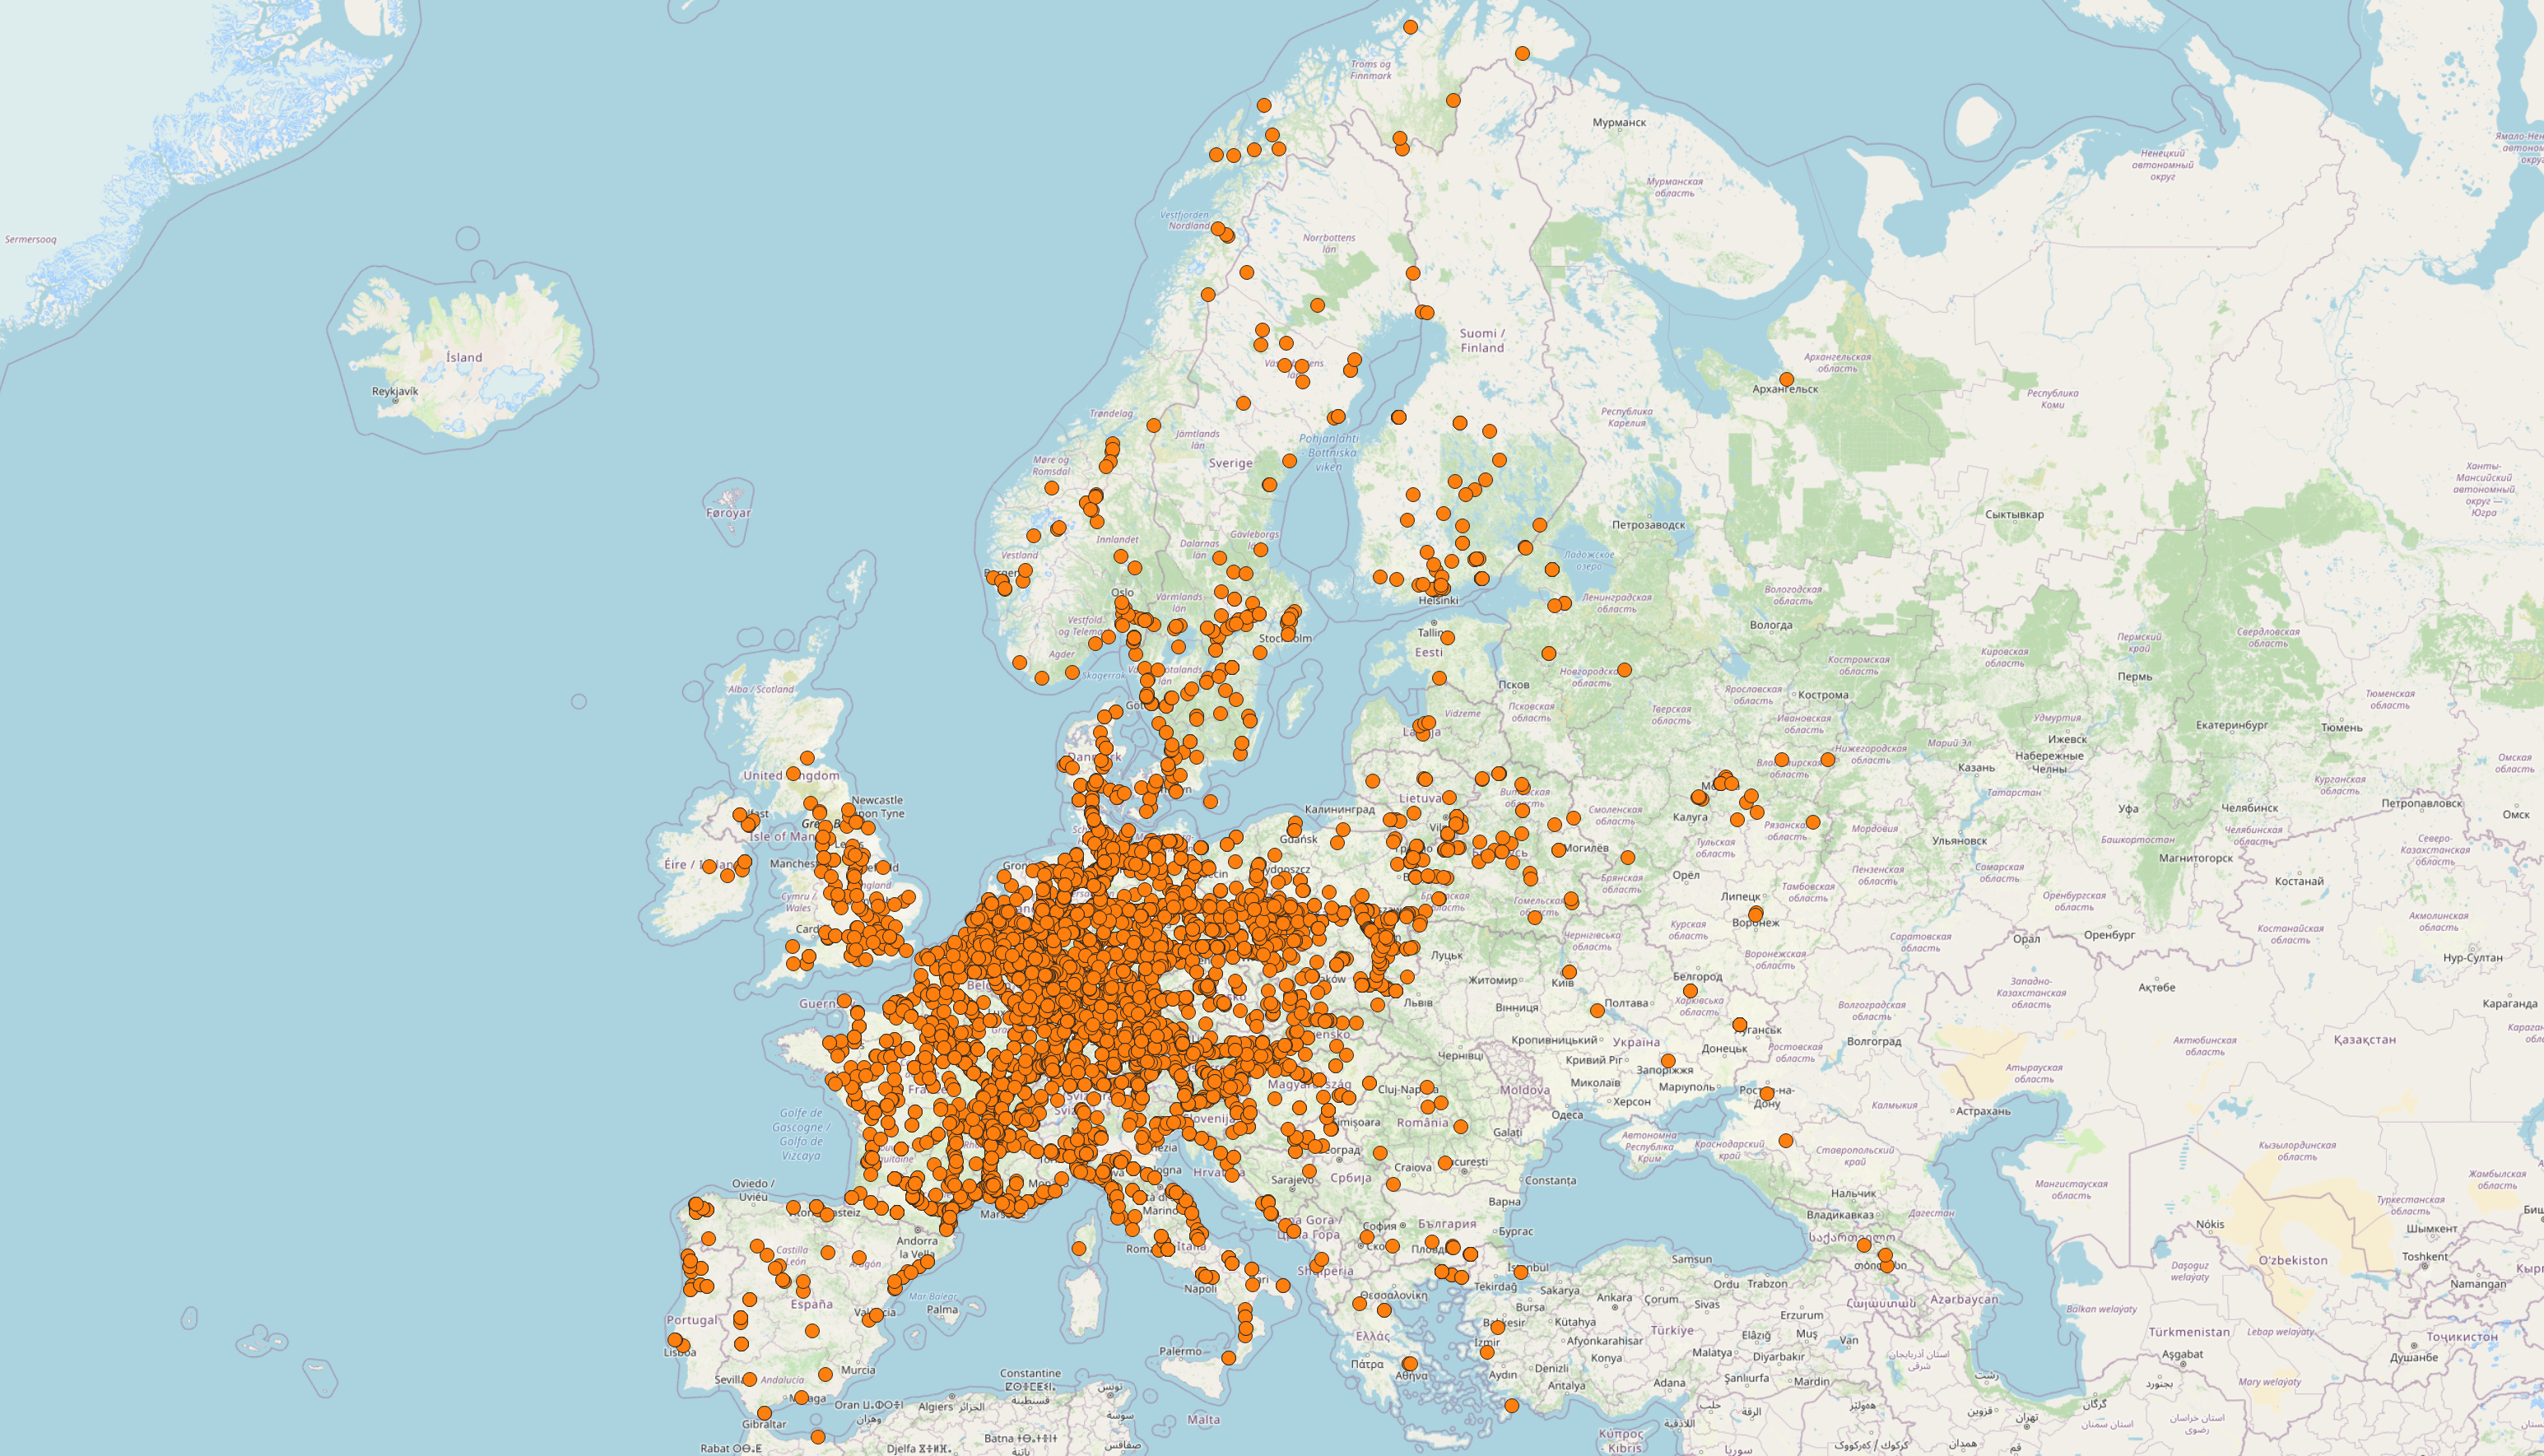
\includegraphics[width=.48\textwidth]{figures/parking_all_europe.png}
		\label{fig:parking_europe_qgis}
	}\hfill
	\subfigure[Highways networks become visible since many designated HGV parking locations are close to a highway]{
		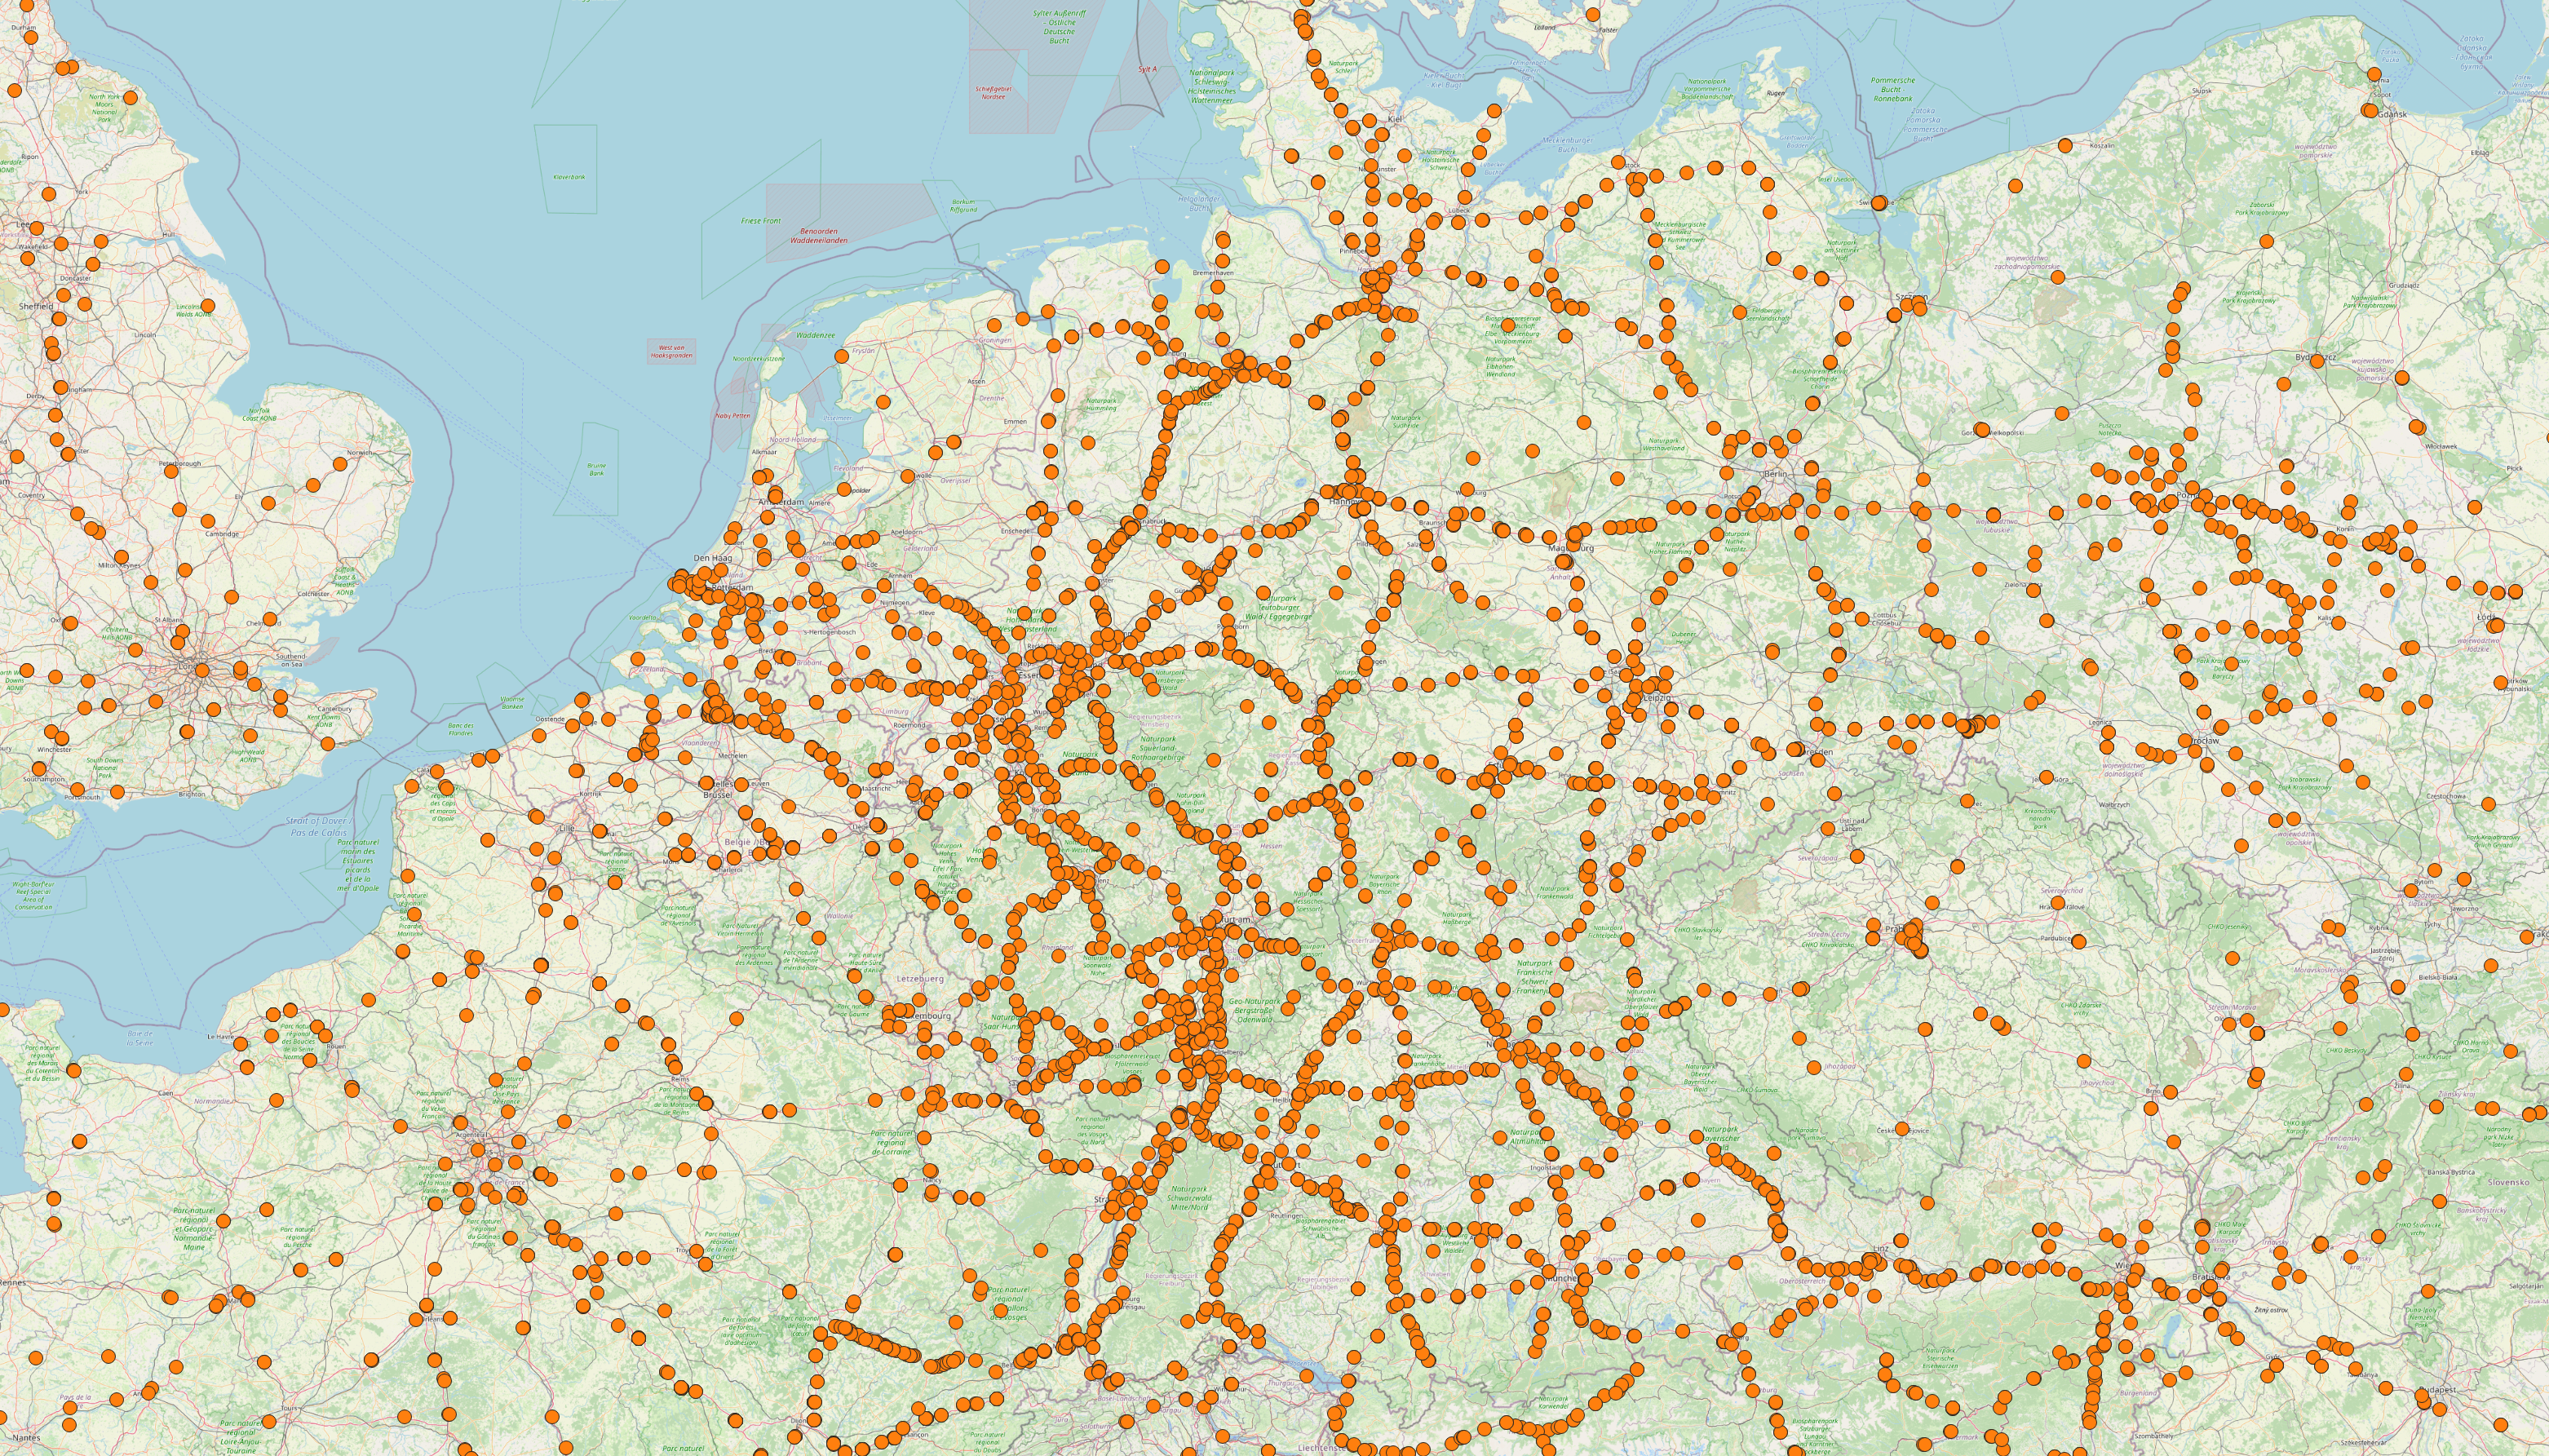
\includegraphics[width=.48\textwidth]{figures/parking_central_europe.png}
		\label{fig:parking_central_europe_qgis}
	}
	\caption{Parking set of designated HGV parking locations which was extracted from OSM data of Europe.}
	\label{fig:parking_qgis}
\end{figure}

We consider OSM nodes and OSM ways as potential parking areas. If an OSM node is found which is marked as HGV parking, we simply flag it as a routing node so that RoutingKit does not remove it from the graph even if it would consider it a modelling node only. Additionally, we add a parking flag for all parking nodes. Some parking areas are modelled as an area instead of a node. In this case, an OSM way which encloses the parking area is flagged as HGV parking. We need to define parking nodes ourselves which we then can add to the routing graph. Additionally, we have to connect these nodes to the rest of the routing graph in order to allow routing from and to them. As a pragmatic solution, we search for OSM nodes on the OSM way modelling the parking area that are part of a second OSM way which is marked as suitable for driving with a car. We flag all of these nodes as routing nodes and parking nodes. RoutingKit will include them in the routing graph. As a result, a parking area which is modelled using an OSM way can result in multiple parking nodes in the routing graph, each of which can be viewed as an entry or exit node. In the routing algorithm, this does not lead to noteworthy overhead since the label which took a break at the exit node of the route through the parking area will always dominate labels which took a break at any entry node. The amount of labels being propagated therefore does not increase significantly.


\subparagraph{Methodology.} All experiments are run sequentially. We conduct experiments regarding the preprocessing time of the core CH and the running time of queries on the extracted routing graph. We average preprocessing running times over \num{10} runs and running times of $s$-$t$ queries over \num{1000} queries with $s$ and $t$ independently chosen uniformly at random for each query. If not stated otherwise, we use $\restr_1$ with $\restr_1^d = \SI{4.5}{\hour}$ and $\restr_1^b = \SI{0.75}{\hour}$ and $\restr_2$ with $\restr_2^d = \SI{9}{\hour}$ and $\restr_2^b = \SI{11}{\hour}$ to approximate the regulations of the EU.

\section{Algorithms}
We evaluate the different algorithms of Chapter~\ref{ch:Algorithm} and the backward pruning of Section~\ref{section:impl}.

As Table \ref{tbl:extensions_runtime} shows, on the German road network, the baseline Dijkstra's algorithm with our amendments for driving time constraints averages at about \SI{30}{\second} of running time. Its bidirectional counterpart without goal-direction almost cuts this running time in half. The goal-directed, unidirectional algorithm on the other hand performs two orders of magnitude better than the baseline, the bidirectional variant of the goal-directed searches even manages to improve the running time by another two orders of magnitude. The goal-directed core CH exhibits the best running times of all algorithms, improving the baseline by a factor of about \num{10000} and even slightly outperforming the bidirectional goal-directed algorithm. The non-goal-directed core CH variant falls back significantly behind its goal-directed counterpart with running times still significantly better than the unidirectional goal-directed algorithm.

On the European road network, we omitted the baseline and the TDRP-2DTC run of the pure goal-directed variants without a core CH since they are too slow or suffer from outliers and would render the experiment impracticable. It appears that the goal-directed variant of the algorithm does not scale very well with longer routes which need an increasing amount of necessary breaks. Most of the performance gain of the goal-directed search in comparison to the baseline originates from the very tight lower-bound given by the CH potentials. If the shortest travel time between two nodes $s$ and $t$ is much larger than $\distance(s,t)$ due to necessary breaks and detours to parking nodes on the route, then the performance of the goal-directed search degrades. The bidirectional variant can mitigate this disadvantage to a certain degree since it connects two routes which each have fewer breaks on the route.

Both core CH algorithms scale better. The simple core CH algorithm scales the best of all algorithms and the goal-directed core CH variant again shows the best result. The core CH variants also show robustness against adding a second driving time constraint on both road networks.

\begin{table}[btp]
	\centering
	\begin{tabular}{cccrrrr}
	\toprule
	              &               &         & \multicolumn{2}{c}{Running Time [\si{\milli\second}]}            \\
	Goal-Directed & Bidirectional & Core CH & 1-DTC                                                 & 2-DTC    \\
	\midrule
	\xmark        & \xmark        & \xmark  & 35110.14                                              & 35110.14 \\
	\cmark        & \xmark        & \xmark  & 1393.72                                               & 1393.72  \\
	\xmark        & \cmark        & \xmark  & 50463.27                                              & 50463.27 \\
	\cmark        & \cmark        & \xmark  & 4.38                                                  & 4.38     \\
	\xmark        & \cmark        & \cmark  & 121.29                                                & 121.29   \\
	\cmark        & \cmark        & \cmark  & 3.47                                                  & 3.47     \\
	\bottomrule
\end{tabular}
	\caption{Average running times of random queries on a German and European road network with one or two driving time constraints.}
	\label{tbl:extensions_runtime}
\end{table}

We also provide the median running times in Table~\ref{tbl:extensions_runtime_median} since the average running time can be skewed significantly due to a few outliers which especially is the case for the goal-directed variants without a core CH. While the running times of non-goal-directed variants improve a little, the median of the running times of goal-directed variants is much smaller than the average in some cases. The core CH shrinks the maximal possible search space in the worst case from the entire graph to much fewer nodes that are reachable via upward edges or are core nodes. Therefore, the outliers are not as bad as for the variants without a core CH.

\begin{table}[hbtp]
	\centering
	\begin{tabular}{cccrrrrrr}
	\toprule
	              &               &         & \multicolumn{2}{c}{Germany [\si{\milli\second}]} & \multicolumn{2}{c}{Europe [\si{\milli\second}]}               \\
	Goal-Directed & Bidirectional & Core CH & 1DTC                                             & 2DTC                                            & 1DTC & 2DTC \\
	\midrule
	\xmark        & \xmark        & \xmark  & 21755.89                                                & 25274.51                                               & -    & -    \\
	\xmark        & \cmark        & \xmark  & 8686.98                                                & 4319.55                                               & -    & -    \\
	\cmark        & \xmark        & \xmark  & 1.53                                                & 1.51                                               & 836.66    & -    \\
	\cmark        & \cmark        & \xmark  & 2.35                                                & 2.00                                               & 1259.19    & -    \\
	\xmark        & \cmark        & \cmark  & 98.57                                                & 137.57                                               & 11.78    & 22.85    \\
	\cmark        & \cmark        & \cmark  & 2.91                                                & 2.93                                               & 9.66    & 10.81    \\
	\bottomrule
\end{tabular}
	\caption{Median running times of random queries on a German and European road network with one or two driving time constraints.}
	\label{tbl:extensions_runtime_median}
\end{table}

We investigate the impact of an increased route length and amount of necessary breaks on a route further. For this, we plot the running times of queries to target nodes of increasing Dijkstra rank on the European road network. The Dijkstra rank is obtained from the sequence in which a standard Dijkstra search without driving time constraints settles its nodes. The Dijkstra rank of a node is the position of the node in that sequence. We plot running times to nodes of rank $2^{10}$, $2^{11}$,\dots,$2^{\log(|V|)}$ where $|V|$ is the number of nodes in the graph. The plot is shown in Figure~\ref{fig:rank_times} with a side-by-side comparison of the unidirectional goal-directed and the goal-directed core CH algorithms.

We first compare the running times with one driving time constraint (TDRP-1DTC) in Figure~\ref{fig:rank_times_1dtc}. The goal-directed algorithm shows an increase of running time of multiple orders of magnitude for large Dijkstra ranks. Starting at Dijkstra rank $2^{20}$, a significant amount of very slow queries occurs which stretches the interquartile range. The median remains low, almost at the first quartile, an indication that the stretching of the IQR is caused by a few very slow queries. The median of the running time jumps from about \SI{2}{\milli\second} at Dijkstra rank $2^{22}$ to about \SI{230}{\milli\second} at Dijkstra rank $2^{23}$. This coincides with the median travel time of the route crossing the mark of \SI{4.5}{\hour} which is the maximum allowed driving time without a break of the shorter driving time constraint of the EU rules being used. Therefore, most queries to target nodes with a Dijkstra rank of $2^{23}$ need at least one break while most queries to target nodes of Dijkstra rank  $2^{22}$ do not need to pause on the route yet. The goal-directed core CH variant scales better with longer queries. It falls slightly behind the goal-directed algorithm for lower Dijkstra ranks due to a larger overhead. While the algorithm suffers from the same general problem of an increasing running time with an increasing route length and number of breaks, the median of its running time increases only by one order of magnitude for the longest queries. The median of the running time only exceeds \SI{10}{\milli\second} at a Dijkstra rank of $2^{24}$ or $2^{25}$ and it never exceeds \SI{12}{\milli\second} at all.

The running times for two driving time constraints (TDRP-2DTC) show a similar picture. In general, the median rises earlier and higher due to a higher number of labels that must be handled by the algorithm in the label sets since at each parking node, a label is tripled instead of doubled. The median of the goal-directed CH nevertheless never exceeds \SI{100}{\milli\second} and there is no single query which ran longer than one second. Another difference is the point at which the median of the goal-directed core CH variant yields a better running time than the median of the pure goal-directed variant. With one driving time constraint, this happens at the Dijkstra rank of $2^{23}$ when most queries need a break on their route. For two driving time constraints this happens earlier at Dijkstra rank $2^{21}$.

\begin{figure}[hbtp]
	\centering
	\subfigure[Goal-Directed and Goal-Directed Core CH Algorithms (TDRP-1DTC)]{
		\includegraphics[width=.95\textwidth]{plots/thesis_rank_times-csp-parking_europe_hgv.png}
		\label{fig:rank_times_1dtc}
	}
	\subfigure[Goal-Directed and Goal-Directed Core CH Algorithms (TDRP-2DTC)]{
		\includegraphics[width=.95\textwidth]{plots/thesis_rank_times-csp_2-parking_europe_hgv.png}
		\label{fig:rank_times_2dtc}
	}
	\caption[Running times of queries to target nodes of increasing Dijkstra rank, logarithmic scales.]{Running times of queries to target nodes of increasing Dijkstra rank, logarithmic scales. The box represents the interquartile range (IQR) from the first quartile Q1 to the third quartile Q3. The horizontal line within the IQR is the median. The whiskers represent the range from $\text{Q1} - \text{IQR} \cdot 1.5$ to $\text{Q3} + \text{IQR} \cdot 1.5$ which contains $99.3\%$ of the data points.}
	\label{fig:rank_times}
\end{figure}

The running times of Figure~\ref{fig:rank_times} to increasingly distant target nodes support the median running times of Table~\ref{tbl:extensions_runtime_median}, but they cannot explain the high average running times of Table~\ref{tbl:extensions_runtime}. The reason for this is that many of the outliers are queries for which no route is found. In fact, when exemplary investigating the $10\%$ of the slowest queries of the goal-directed algorithm, we find that two thirds of those did not find a route. These queries are naturally left out when plotting queries to nodes for which a Dijkstra rank exists. The remaining queries are long queries with a high number of breaks on the route. To complete the evaluation of the different variants of the algorithm, we provide the running times on the European road network of the queries for which no route was found in Table~\ref{tbl:times_no_path}.

\begin{table}[hbtp]
	\centering
	\begin{tabular}{cccrrrrrr}
	\toprule
	              &               &         & \multicolumn{2}{c}{Mean [\si{\milli\second}]} & \multicolumn{2}{c}{Median [\si{\milli\second}]}                 \\
	Goal-Directed & Bidirectional & Core CH & 1-DTC                                       & 2-DTC                                         & 1-DTC & 2-DTC \\
	\midrule
	\xmark        & \xmark        & \xmark  & -                                           & -                                             & -     & -     \\
	\cmark        & \xmark        & \xmark  & 167739.69                                           & 1384.01                                             & 9758.52     & 265.06     \\
	\xmark        & \cmark        & \xmark  & -                                           & -                                             & -     & -     \\
	\cmark        & \cmark        & \xmark  & 14168.37                                           & 397.66                                             & 7532.67     & 542.91     \\
	\xmark        & \cmark        & \cmark  & 321.22                                           & -                                             & 346.76     & -     \\
	\cmark        & \cmark        & \cmark  & 220.41                                           & -                                             & 245.75     & -     \\
	\bottomrule
\end{tabular}
	\caption{Comparison of running times of queries which failed to find a feasible route.}
	\label{tbl:times_no_path}
\end{table}

Finally, we evaluate the backward pruning as defined in Algorithm~\ref{alg:bw_pruning} in use with the goal-directed core CH algorithm on the European road network. For this experiment, we average running times of \num{10000} queries. Table~\ref{tbl:opt_runtime} shows that the pruning can lead to an improvement of the running time. TODO weird sample, increase n

\begin{table}[hbtp]
	\centering
	\begin{tabular}{crrrr}
	\toprule
	                 & \multicolumn{2}{c}{Mean [\si{\milli\second}]} & \multicolumn{2}{c}{Median [\si{\milli\second}]}                 \\
	Backward Pruning & 1-DTC                                         & 2-DTC                                           & 1-DTC & 2-DTC \\
	\midrule
	\xmark           & 131.89                                             & 262.37                                               & 45.04     & 27.10     \\
	\cmark           & 115.20                                             & 235.18                                               & 36.14     & 24.64     \\
	\bottomrule
\end{tabular}

	\caption{Comparison of running times of the goal-directed core CH algorithm with and without the backward pruning of Section~\ref{section:impl}.}
	\label{tbl:opt_runtime}
\end{table}

\section{Influence of Parameters and Data}
In this section, we investigate how varying parameters and changes in the road network influence the running time of our algorithms. The European road network is used for all experiments. W compare the non-goal-directed and goal-directed core CH variants to be able to observe the effect of the goal-direction.

\subsection{Driving Time Constraints}
We investigate how different driving time limits and break times influence the running time of the goal-directed core CH and non-goal-directed core CH algorithms. We use only one driving time constraint $\restr$ (1DTC) to be able to change one parameter at a time and observe the consequences. Figure~\ref{fig:eval_driving_time} shows the running times for an increasing maximum allowed driving time $\restr^d$. We plot the median of 1000 random queries for one value of $c^d$ and increase the driving time limit stepwise. Additionally, the plot is smoothed using a rolling window mean to increase readability. To ease the comparistion of both plots, the scaling of the y-axis is the same in both plots.

The goal-directed core CH variant behaves differently compared to the core CH variant, except for very small driving time limits when both variants fail to find a path and terminate early. When increasing the driving time limit, the search radius first increases equally for both. This is because the goal-directed variant presents no advantage over the non-goal-directed variant if a route from $s$ to $t$ is not found because of the driving time constraint. The goal-directed algorithm can exclude nodes $v$ from the search only if the target node $t$ is not reachable from the $v$ at all in the graph, since the CH-Potentials yield an infinite distance value in this case. It fails to do so if $t$ is reachable from $s$ in the graph, but the driving time constraint prohibits finding a feasible route. In this case, both algorithms settled the same labels, just in a different order. This behavior changes when the driving time limit increased enough that a route can be found and the advantage of the goal-directed algorithm becomes apparent. In the optimal case, which is if a route from a node $v$ to $t$ without the need for a break exists, the CH-Potentials yield the exact distant values $\distance(v,t)$. Therefore, the goal-directed algorithm knows the shortest path to $t$ and does not search aside the shortest route.

\begin{figure}[hbtp]
	\centering
	\subfigure[Core CH Algorithm]{
		\includegraphics[width=.48\textwidth]{plots/thesis_driving_times-csp-parking_europe_hgv-core_ch-time_ms.png}
		\label{fig:eval_driving_time_core_ch}
	}\hfill
	\subfigure[Goal-Directed Core CH Algorithm]{
		\includegraphics[width=.48\textwidth]{plots/thesis_driving_times-csp-parking_europe_hgv-core_ch_chpot-time_ms.png}
		\label{fig:eval_driving_time_gd_core_ch}
	}
	\caption{Running time means and IQR of the core CH and the goal-directed core CH algorithms with increasing maximum allowed driving time.}
	\label{fig:eval_driving_time}
\end{figure}

Second, we vary the break time $\restr^b$ of the driving time constraint in the same way which we show in Figure~\ref{fig:eval_break_time}. If the break time is exactly zero, there never are multiple labels at a parking node. When duplicating a label at a parking node to represent the two options of taking a break and not taking a break, the label $l$ which took the break will always dominate the other label $l'$ since it resets the distance since the last break to zero without adding any break time to its travel time.

In the non-goal-directed case, the labels in the label queue are sorted using their travel time. A label $l$ at a parking node $v$ which takes the break is inserted into the queue at a position further back than the label $l'$ that does not take a break. The search does not settle $l$ at all if the break time which has been added to its travel time increased its travel time over the travel time of the shortest route from $s$ to $t$. If the label $l$ is part of the shortest route, the algorithm spends unnecessary time with propagating labels which have taken fewer breaks and therefore yield a smaller travel time, but will not reach $t$ because they exceed the driving time limit before. The longer the break time, the more of such labels are settled before $l$ which increases the running time. The running time stops to increase when there are no more labels with fewer breaks which the algorithm can propagate before $l$. In this case, the algorithm first propagates all labels which take zero breaks, then all labels which take one break and so on until a feasible route to $t$ can be found. As Figure~\ref{fig:eval_break_time_core_ch} shows, this is already the case after a small increase of the break time from zero. Many break time values from real-world regulations fall into this range in which the running time increases significantly with an increasing break time. For example, the US HOS regulations include a break time of \SI{30}{\minute} and the EU driver's working hours regulations include a break time of \SI{45}{\minute}.

In the goal-directed case, the labels are sorted in the queue using the sum of their travel time and the potential towards the target node. If a label is positioned further back in the queue, it takes a longer detour from the route which the CH-Potentials have determined to be the shortest route without regard for driving time constraints to $t$. Detours arise from the need to deviate from the direct route to reach a parking node because the direct route exceeded the driving time limit. As a consequence, the algorithm starts to propagate labels along the direct route until either $t$ is found or the driving time limit is exceeded. It then continues to do so with the label that took the smallest detour. If a label takes a break it only gets positioned further back in the label queue if the break is not of use, i.e., if the break does not spare a break on the remaining route. Such labels cannot be part of a shortest route. Therefore, the break time has no influence on the running time of the algorithm, a finding which is also supported by the large IQR.

\begin{figure}[hbtp]
	\centering
	\subfigure[Core CH Algorithm]{
		\includegraphics[width=.48\textwidth]{plots/thesis_break_times-csp-parking_europe_hgv-core_ch-time_ms.png}
		\label{fig:eval_break_time_core_ch}
	}\hfill
	\subfigure[Goal-Directed Core CH Algorithm]{
		\includegraphics[width=.48\textwidth]{plots/thesis_break_times-csp-parking_europe_hgv-core_ch_chpot-time_ms.png}
		\label{fig:eval_break_time_gd_core_ch}
	}
	\caption{Running time means and IQR of the core CH and the goal-directed core CH algorithms with an increasing break time.}
	\label{fig:eval_break_time}
\end{figure}


\subsection{Parking Set of the Road Network}\label{sec:parking_set_exp}
We investigate how changes to set of parking nodes $P$ influence the running time of the goal-directed core CH algorithm. We extend our standard set of designated HGV parking locations to a set which includes all parking locations and thus is way larger. The parking locations are included in $P$ if  \texttt{amenity = "parking"} or the tag \texttt{parking} exists with any value. For this choice of $P$, we set the core size to $5\%$ of the total numbers of nodes in the European road network which is the smallest practicable core size in this case due to the construction time of the core CH. We include a reference run using HGV parking nodes using the same core size. Additionally, we run an experiment in which we use a set of charging station locations for $P$, instead of parking nodes. Charging stations are extracted from the OSM data if \texttt{amenity = "charging\_station"} or \texttt{parking = "charging"} and at the same time, if the OSM object has a tag \texttt{bicycle}, it must not be \texttt{bicycle = "yes"}.

TODO describe with new data

\begin{table}[hbtp]
	\centering
	\begin{tabular}{rrrrrr}
	\toprule
	                    &                       & \multicolumn{2}{c}{Mean [\si{\milli\second}]} & \multicolumn{2}{c}{Median [\si{\milli\second}]}               \\
	Type of Set $P$     & Number of Nodes $|C|$ & 1DTC                                          & 2DTC                                            & 1DTC & 2DTC \\
	\midrule
	HGV Parking         & 6796                     & 9.82                                             & 14.65                                               & 8.50    & 9.93    \\
	Charging Stations   & 56011                     & 3.79                                             & 4.92                                               & 3.52    & 3.98    \\
	Any Parking ($5\%$) & 4124476                     & 2.88                                             & 3.01                                               & 2.75    & 2.83    \\
	HGV Parking ($5\%$) & 4075286                     & 2.01                                             & 2.01                                               & 1.97    & 1.98    \\
	\bottomrule
\end{tabular}
	\caption{Comparison of running times of the goal-directed core CH algorithm with different choices for the set of parking nodes $P$.}
	\label{tbl:parking_set_times}
\end{table}

\subsection{Car and Truck Speeds}
RoutingKit assumes speeds for different kinds of OSM ways reaching from \SI[per-mode = symbol]{5}{\kilo\meter\per\hour} for walking speed to \SI[per-mode = symbol]{130}{\kilo\meter\per\hour} on highways. The assumed highway speeds are faster than the possible or allowed speed of HGV. In this experiment, we measure the running time of the goal-directed core CH algorithm in multiple iterations in which we cap the maximum speed at the values \SI[per-mode = symbol]{130}{\kilo\meter\per\hour} (standard RoutingKit setting), \SI[per-mode = symbol]{100}{\kilo\meter\per\hour}, \SI[per-mode = symbol]{80}{\kilo\meter\per\hour} (common maximum truck speed), \SI[per-mode = symbol]{50}{\kilo\meter\per\hour}, \SI[per-mode = symbol]{30}{\kilo\meter\per\hour}, and \SI[per-mode = symbol]{15}{\kilo\meter\per\hour} and observe the change in running time. We plot the average running time of \num{10000} random queries in each iteration.

First, the running time begins to increase when the maximum assumed speed of a vehicle is capped at lower speeds. This can be explained by the degrading hierarchy of the road network which leads to a weaker core CH. At a maximum speed of around \SI[per-mode = symbol]{50}{\kilo\meter\per\hour}, the running time reaches a high point and begins to decrease again. TODO y

\begin{figure}[hbtp]
	\centering
	\includegraphics[width=.95\textwidth]{plots/thesis_speed_cap.png}
	\label{fig:truck_speed_limit}
	\caption{The running time of goal-directed core CH queries increases with a decreasing speed cap, i.e., a decreasing assumed maximum speed of the vehicle until it reaches a high point and decreases again fir very low speed caps.}
\end{figure}

\section{Core Contraction Hierarchy}
In Section~\ref{section:impl}, we mentioned the possibility of including more nodes than the parking nodes in the core of the core CH. Parking nodes are not necessarily important nodes according to the computed node order of the core CH, but we define them as the most important nodes of the road network regardless which impairs the quality of the core CH. It is beneficial to also include the most important nodes according to the node order in the core. In the following, we will analyze the impact of different core sizes on the running time of queries of the goal-directed core CH algorithm on the European road network. The choice of the core size also significantly impacts the construction time of the core CH.

In Figure~\ref{fig:preprocessing_time_core_ch}, we plot the construction time of the core CH for increasing core sizes in relation to the number of nodes in the graph. The plot shows that the construction time begins to increase drastically for a core size smaller than $0.01\%$ of the nodes.

\begin{figure}[hbtp]
	\centering
	\includegraphics[width=.95\textwidth]{plots/thesis_core_sizes-csp-parking_europe_hgv-constr_time.png}
	\label{fig:preprocessing_time_core_ch}
	\caption{Construction times of the core CH decrease exponentially with an increasing core size relative to the number of nodes in the graph.}
\end{figure}

Figure~\ref{fig:query_time_core_ch_sizes} shows that the average running time of a query decreases with a decreasing core size, but the benefit of contracting more nodes becomes much smaller for very small core sizes. This observation can be used to lower the preprocessing time significantly by including more non-parking nodes in the core without loosing much of the performance of the goal-directed core CH queries. A good trade off in the example with the European road network with HGV parking nodes would choose a core size between $0.1\%$ and $0.01\%$ of the graph's number of nodes. As mentioned in Section~\ref{sec:parking_set_exp}, certain sets of core nodes cause high node degrees at an early stage during the contraction of nodes. Allowing additional nodes in the core might be the only feasible approach to build a core CH in those cases since the node degrees become too high to be able to finish the contraction of all non-parking nodes in practicable time.

\begin{figure}[hbtp]
	\centering
	\includegraphics[width=.95\textwidth]{plots/thesis_core_sizes-csp-parking_europe_hgv-time_ms.png}
	\label{fig:query_time_core_ch_sizes}
	\caption{Running time of goal-directed core CH queries for varying core sizes relative to the number of nodes in the graph.}
\end{figure}
